\chapter{Linear Classification at the Top}\label{chap: linear}

In this chapter, we focus on the special case when the model~$f$ is linear
\begin{equation*}
  f(\bm{x}; \bm{w}) = \bm{w}^{\top} \bm{x},
\end{equation*}
where~$\bm{w} \in \R^d$ is the normal vector to the separating hyperplane. In such a case, the framework~\eqref{eq: aatp surrogate} simplifies into the following form
\begin{mini*}{\bm{w}}{
  \frac{1}{2} \norm{\bm{w}}^2 + \lambda_1 \cdot \fps(\bm{s}, t) + \lambda_2 \cdot \fns(\bm{s}, t)
  }{}{}
  \addConstraint{s_i}{= \bm{w}^{\top} \bm{x}_i, \quad i \in \I}
  \addConstraint{t}{= G(\Brac[c]{\bm{s}_i; y_i}_{i \in \I}).}
\end{mini*}

In this chapter, we provide a theoretical analysis of the unified framework from Chapter~\ref{chap: framework} with linear classifier. We consider purely the problem \textit{formulations} and not individual \textit{algorithms} which specify how to solve these formulations. The overview of all formulations that falls into the framework~\eqref{eq: aatp surrogate} is in Table~\ref{tab: summary formulations}. We focus mainly on the following desirable properties:
\begin{itemize}
  \item \textit{Convexity} implies a guaranteed convergence for many optimization algorithms or their better convergence rates~\cite{boyd2004convex}.
  \item \textit{Differentiability} increases the speed of convergence.
  \item \textit{Stability} is a general term, by which we mean that the global minimum is not at~$\bm{w} = \bm{0}$. This actually happens for many formulations from Chapter~\ref{chap: framework} and results in the situation where the separating hyperplane is degenerate and does not actually exist.
\end{itemize}
For a nicer flow of text, we postpone the proofs to Appendix~\ref{chap: linear}. Moreover, we show the results only for formulations from Section~\ref{sec: ranking} and~\ref{sec: aatp}. The results for methods from Section~\ref{sec: Neyman-Pearson} are identical to the one for methods in Section~\ref{sec: aatp}. 

\section{Convexity}\label{sec: convexity}

Convexity is one of the most important properties in numerical optimization. It ensures that the optimization problem has neither stationary points nor local minima. All points of interest are global minima. Moreover, it allows for faster convergence rates. Before we present any results, we recall the form of the decision threshold from Section~\ref{sec: aatp}
\begin{equation*}
  \begin{aligned}
    t_1(\bm{w}) & = \max \Set{t}{\frac{1}{n} \sum_{i \in \I} \Iverson{s_i \geq t} \geq \tau} \\
    t_2(\bm{w}) & = \frac{1}{K} \sum_{i=1}^{K} s_{[i]} \\
    t_3(\bm{w}) & \quad \text{solves} \quad \frac{1}{n} \sum_{i \in \I} l\Brac{\vartheta(s_i - t)} = \tau, \\
  \end{aligned}
\end{equation*}
where we use Notation~\ref{not: scores}. Note that we denote the thresholds as functions of weights. This is true, since the scores~$\bm{s}$ depends on the weights~$\bm{w}.$ The first result is summarized in the following proposition.

\begin{restatable}{proposition}{propconvex}\label{prop:convex}
  Thresholds~$t_2$ from~\eqref{eq: aatp quantile mean} and~$t_3$ from~\eqref{eq: aatp quantile surrogate} are convex functions of the weights~$\bm{w}$. The threshold function~$t_1$ from~\eqref{eq: aatp quantile} is non-convex.
\end{restatable}

\noindent The proposition says, that formulation \Grill uses non-convex threshold with respect to weights~$\bm{w}$ while formulations \TopMeanK, \PatMat use the convex ones. Moreover, since \tauFPL and \TopPushK formulations use almost the same threshold as \TopMeanK, but computed only from negative scores, the resulting threshold is also convex function of weights. The same holds for formulations \PatMat and \PatMatNP. Finally, the threshold for \TopPush formulation is convex since maximum is convex function. The next theorem shows which formulations are convex.

\begin{restatable}{theorem}{thmconvex}\label{thm:convex}
  If the threshold~$t = t(\bm{w})$ is a convex function of the weights~$\bm{w}$, then function
  \begin{equation*}
    L(\bm{w}) = \fns(\bm{s}, t)
  \end{equation*}
  is convex.
\end{restatable}

\noindent While the proof of Theorem~\ref{thm:convex} is simple, it points to the necessity of considering only false-negatives in the objective of the formulations in Chapter~\ref{chap: framework}. In such a case, \TopPush, \TopPushK, \TopMeanK, \tauFPL, \PatMat and \PatMatNP are convex problems. At the same time, \Grill and \GrillNP are not convex problems.

\section{Differentiability}

Similarly to convexity, differentiability allows for faster convergence rate and in some algorithms, better termination criteria. The next theorem shows which formulations are differentiable.

\begin{restatable}{theorem}{derivative}\label{thm:derivative}
  If the surrogate function~$l$ is differentiable, then threshold~$t_3$ is a differentiable function of the weights~$\bm{w}$ and its derivative equals to
  \begin{equation*}
    \nabla t_3(\bm{w}) = \frac{\sum_{i \in \I} l'\Brac{\vartheta(\bm{w}^{\top} \bm{x}_i - t_3(\bm{w}))}\bm{x}_i}{\sum_{i \in \I}l'\Brac{\vartheta(\bm{w}^{\top} \bm{x}_i - t_3(\bm{w}))}}.
  \end{equation*}
  The threshold functions~$t_1$ and~$t_2$ are non-differentiable.
\end{restatable}

\noindent This theorem shows that the objective functions of \PatMat and \PatMatNP are differentiable. This allows us to prove the convergence of the stochastic gradient descent for these two formulations in Section~\ref{sec:convergence}.

\section{Stability}\label{sec: stability}

We first provide a simple example and show that many formulations from Table~\ref{tab: summary formulations} are degenerate for it. Then we analyze general conditions under which this degenerate behaviour happens.

\begin{restatable}[Degenerate Behaviour]{example}{degeneratebehavior}\label{ex: degenerate behaviour}
  We consider~$n$ negative samples uniformly distributed in~$[-1,0]\times[-1,1]$,~$n$ positive samples uniformly distributed in~$[0,1]\times[-1,1]$ and one negative sample at~$(2,0)$, see Figure~\ref{fig: degenerate behaviour} (left). We consider the hinge loss and no regularization. If~$n$ is large, the point at~$(2,0)$ is an outlier and the dataset is separable and the separating hyperplane has the normal vector~$\bm{w}=(1,0)$. 
\end{restatable}

\noindent Table~\ref{tab:example} shows the threshold~$t$ and the objective value~$L$ for two points~$\bm{w}_0=(0,0)$ and~$\bm{w}_0=(1,0)$. These two points are both important:~$\bm{w}_0$ does not generate any separating hyperplane, while~$\bm{w}_1$ generates the optimal separating hyperplane. We show the precise computation in Appendix~\ref{app: stability}. Since the dataset is perfectly separable by~$\bm{w}_0$, we expect that~$\bm{w}_0$ provides a lower objective than~$\bm{w}_0$. By highlithing the better objective in Table~\ref{tab:example} by green, we see that this did not happen for \TopPush and \TopMeanK. It can be shown that~$\bm{w}_0$ is even the global minimum for \TopPush and \TopMeanK. This raises the question of whether some tricks, such as early stopping or excluding a small ball around zero, cannot overcome this difficulty. The answer is negative as shown in Figure~\ref{fig: degenerate behaviour} (right). Here, we run \TopPush from several starting points, and it always converges to zero from one of the three possible directions; all of them far from the normal vector to the separating hyperplane.

\begin{figure}
  \centering
  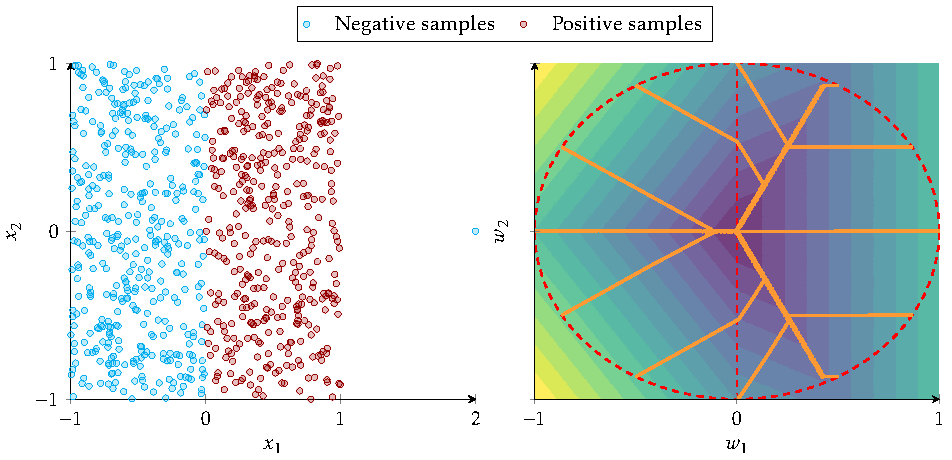
\includegraphics[width=\linewidth]{images/toppush_convergence.pdf}
  \caption{Left: distribution of positive (red circles) and negative samples (blue circles) for the example from Example~\ref{ex: degenerate behaviour} Right: contour plot of the objective function value for \TopPush and its convergence (orange lines) to the zero vector from~$12$ initial points.}
  \label{fig: degenerate behaviour}
\end{figure}

\begin{table}
  \centering
  \begin{NiceTabular}{lccccc}
    \toprule
    \Block{2-1}{\textbf{Name}}
      & \Block{2-1}{\textbf{Label}}
      & \Block{1-2}{$\bm{w}_0=(0,0)$}
      && \Block{1-2}{$\bm{w}_0=(1,0)$} \\
    \cmidrule(lr){3-4} \cmidrule(lr){5-6}
    & & $t$
      & $L$
      & $t$
      & $L$ \\
    \midrule
    \TopPush
      & \eqref{eq: toppush surrogate}
      & $0$
      & \Block[fill=mygreen!50]{1-1}{$1$}
      & $2$
      & $2.5$ \\
    \TopPushK
      & \eqref{eq: toppushK surrogate}
      & $0$
      & $1$
      & $\frac{2}{K}$
      & \Block[fill=mygreen!50]{1-1}{$0.5+\frac{2}{K}$} \\
    \midrule
    \Grill
      & \eqref{eq: grill}
      & $0$
      & $2$
      & $1-2\tau$
      & \Block[fill=mygreen!50]{1-1}{$1.5+2\tau(1-\tau)$} \\
    \TopMeanK
      & \eqref{eq: topmeank}
      & $0$
      & \Block[fill=mygreen!50]{1-1}{$1$}
      & $1-\tau$
      & $1.5-\tau$ \\
    \PatMat
      & \eqref{eq: patmat}
      & $\frac{1}{\vartheta}(1-\tau)$
      & $1+\frac{1}{\vartheta}(1-\tau)$
      & $\frac{1}{\vartheta}(1-\tau)$
      & \Block[fill=mygreen!50]{1-1}{$0.5 + \frac{1}{\vartheta}(1-\tau)$} \\
    \bottomrule
  \end{NiceTabular}
  \caption{Comparison of formulations on the very simple problem from Section~\ref{sec: stability}. Two formulations have the global minimum (denoted by green color) at~$\bm{w}_0=(0,0)$ which does not generate any separating hyperplane. The optimal separating hyperplane is generated by~$\bm{w}_1=(1,0)$.}
  \label{tab:example}
\end{table}

The convexity derived in the previous section guarantees that there are no local minima. However, as we showed in the example above, the global minimum may be at~$\bm{w} = \bm{0}$. This is highly undesirable since~$\bm{w}$ is the normal vector to the separating hyperplane and the zero vector provides no information. In the rest of the section, we analyze when this situation happens. The first result states that if the decision threshold~$t = t(\bm{w})$ is above a certain value, then zero has a better objective that~$\bm{w}$. If this happens for all~$\bm{w}$, then zero is the global minimum.
\begin{restatable}{theorem}{larget}\label{thm:large_t}
  Consider any of these formulations: \TopPush, \TopPushK, \TopMeanK or \tauFPL. Fix any~$\bm{w}$ and denote the corresponding objective function~$L(\bm{w})$ and threshold~$t(\bm{w})$. If we have
  \begin{equation}\label{eq:w_zero_nn}
    t(\bm{w})\geq \frac{1}{\npos} \sum_{i \in \Ipos} \bm{w}^{\top} \bm{x}_i,
  \end{equation}
  then~$L(\bm{0}) \leq L(\bm{w})$. Specifically, using notation~\ref{not: scores} we get the following implications
  \begin{equation}\label{eq:w_zero}
    \begin{aligned}
    s_{[1]}^- \geq \frac{1}{\npos} \sum_{i=1}^{\npos} s_{i}^+
      & \implies L(\bm{0}) \leq L(\bm{w}) \text{ for } \TopPush, \\
    \frac{1}{K}\sum_{i=1}^K s_{[i]}^- \geq \frac{1}{\npos} \sum_{i=1}^{\npos} s_{i}^+
      & \implies L(\bm{0}) \leq L(\bm{w}) \text{ for } \TopPushK, \\
    \frac{1}{K} \sum_{i=1}^{K} s_{[i]} \leq \sum_{i=1}^{\npos} s_{i}^+
      & \implies L(\bm{0}) \leq L(\bm{w}) \text{ for } \TopMeanK, \\
    \frac{1}{\nneg\tau} \sum_{i=1}^{\nneg\tau} s_{[i]}^- \geq \frac{1}{\npos}\sum_{i=1}^{\npos} s_{i}^+
      & \implies L(\bm{0}) \leq L(\bm{w}) \text{ for } \tauFPL. \\
    \end{aligned}
  \end{equation}
\end{restatable}

\noindent We can use this result immediately to deduce that some formulations have the global minimum at~$\bm{w} = \bm{0}$. More specifically, \TopPush fails if there are outliers, and \TopMeanK fails whenever there are many positive samples.

\begin{corollary}\label{cor:toppush}
  Consider the \TopPush formulation. If the positive samples lie in the convex hull of negative samples, then~$\bm{w}=\bm{0}$ is the global minimum.
\end{corollary}

\begin{corollary}\label{cor:topmean}
  Consider the \TopMeanK formulation. If~$\npos\geq n\tau$, then~$\bm{w}=\bm{0}$ is the global minimum.
\end{corollary}

\noindent The proof of Theorem~\ref{thm:large_t} employs the fact that all formulations in the theorem statement have only false-negatives in the objective. If~$\bm{w}_0=\bm{0}$, then~$\bm{w}_0^\top \bm{x}_i = 0$ for all~$i \in \I,$ the threshold equals to~$t = 0$ and the objective equals to one. If the threshold is large for~$\bm{w}$, many positives are below the threshold, and the false-negatives have the average surrogate value larger than one. In such a case,~$\bm{w}_0 = \bm{0}$ becomes the global minimum. There are two fixes to this situation:
\begin{itemize}
  \item Include false-positives to the objective. This approach is taken by \Grill and \GrillNP and necessarily results in the loss of convexity as shown in Section~\ref{sec: convexity}.
  \item Move the threshold away from zero even when all scores~$\bm{s}$ are zero. This approach is taken by our formulations \PatMat and \PatMatNP and keeps convexity.
\end{itemize}
The next theorem shows the advantage of the second approach.

\begin{restatable}{theorem}{patmatzero}\label{thm:patmat_zero}
  Consider the \PatMat or \PatMatNP formulation with the hinge surrogate and no regularization. Assume that for some~$\bm{w}$ we have
  \begin{equation}\label{eq:patmat_zero}
    \frac{1}{\npos}\sum_{i \in \Ipos}\bm{w}^{\top} \bm{x}_i > \frac{1}{\nneg}\sum_{j \in \Ineg}\bm{w}^{\top} \bm{x}_j.
  \end{equation}
  Then there is a scaling parameter~$\vartheta_0$ for the surrogate top $\tau$-quantile~\eqref{eq: aatp quantile surrogate} such that~$L(\bm{w}) < L(\bm{0})$ for all~$\vartheta \in (0, \vartheta_0)$.
\end{restatable}

\noindent This theorem shed some light on the behaviour of the formulations. Theorem~\ref{thm:large_t} states that the stability of \tauFPL requires
\begin{equation}\label{eq:stability1}
  \frac{1}{\nneg\tau}\sum_{i=1}^{\nneg\tau}s_{[i]}^- < \frac{1}{\npos}\sum_{i=1}^{\npos} s_{i}^+,
\end{equation}
while Theorem~\ref{thm:patmat_zero} states that the stability of \PatMatNP is ensured by
\begin{equation}\label{eq:stability2}
  \frac{1}{\nneg}\sum_{i=1}^{\nneg}s_{[i]}^- < \frac{1}{\npos}\sum_{i=1}^{\npos} s_{i}^+.
\end{equation}
The right-hand sides of \eqref{eq:stability1} and \eqref{eq:stability2} are the same, while the left-hand side of \eqref{eq:stability2} is always smaller than the left-hand side of \eqref{eq:stability1}. This implies that if \tauFPL is stable, then \PatMatNP is stable as well.

At the same time, there may be a huge difference in the stability of both formulations. Since the scores of positive samples should be above the scores of negative samples, the scores~$\bm{s}$ may be interpreted as performance. Then formula \eqref{eq:stability1} states that if the mean performance of a \emph{small number of the best} negative samples is larger than the average performance of \emph{all} positive samples, then \tauFPL fails. On the other hand, formula \eqref{eq:stability2} states that if the average performance of \emph{all} positive samples is better than the average performance of \emph{all} negative samples, then \PatMatNP is stable. The former may well happen as accuracy at the top is interested in a good performance of only a small number of positive samples.

\section{Convergence of stochastic gradient descent}\label{sec:convergence}

The previous section analyzed the formulations from Chapter~\ref{chap: framework} but did not consider any optimization algorithms. In this section, we show a basic version of the stochastic gradient descent and then show its convergent version. Since due to considering the threshold, gradient computed on a minibatch is a biased estimate of the true gradient, we need to use variance reduction techniques, and the proof is rather complex.

Many optimization algorithms for solving the formulations from Chapter~\ref{chap: framework} use primal-dual or purely dual formulations.~\cite{eban2017scalable} introduced dual variables and used alternating optimization to the resulting min-max problem. ~\cite{li2014top} and~\cite{zhang2018tau} dualized the problem and solved it with the steepest gradient ascent.~\cite{macha2020nonlinear} followed the same path but added kernels to handle non-linearity. We follow the ideas of~\cite{mackey2018constrained} and~\cite{adam2019machine} and solve the problems directly in their primal formulations. Therefore, even though we use the same formulation for \TopPush as~\cite{li2014top} or for \tauFPL as~\cite{zhang2018tau}, our solution process is different. However, due to convexity, both algorithms should converge to the same point.

The decision variables in \eqref{eq: aatp surrogate} are the normal vector of the separating hyperplane~$\bm{w}$ and the threshold~$t$. To apply an efficient optimization method, we need to compute gradients. The simplest idea~\cite{grill2016learning} is to compute the gradient only with respect to~$\bm{w}$ and then recompute~$t$. A more sophisticated way is based on the chain rule. For each~$\bm{w}$, the threshold~$t$ can be computed uniquely. We stress this dependence by writing~$t(\bm{w})$ instead of~$t$. By doing so, we effectively remove the threshold~$t$ from the decision variables and~$\bm{w}$ remains the only decision variable. Note that the convexity is preserved. Then we can compute the derivative via the chain rule
\begin{equation}\label{eq:derivatives}
  \begin{aligned}
  L(\bm{w})
    & = \frac{1}{\npos} \sum_{i \in \Ipos} l(t(\bm{w}) - \bm{w}^{\top} \bm{x}_i) + \frac{\lambda}{2}\norm{\bm{w}}^2, \\
  \nabla L(\bm{w})
    & = \frac{1}{\npos} \sum_{i \in \Ipos} l'(t(\bm{w}) - \bm{w}^{\top} \bm{x}_i)(\nabla t(\bm{w}) - \bm{x}_i) + \lambda \bm{w}.
  \end{aligned}
\end{equation}
The only remaining part is the computation of~$\nabla t(\bm{w})$. It is simple for~$\nabla t_1(\bm{w})$ and~$\nabla t_2(\bm{w})$ and Theorem~\ref{thm:derivative} shows the computation for~$\nabla t_3(\bm{w})$. Moreover, Appendix~\ref{app:threshold} provides an efficient computation method for~$t_3(\bm{w})$. Having derivative \eqref{eq:derivatives}, deriving the stochastic gradient is simple. It partitions the dataset into minibatches and provides an update of the weights~$\bm{w}$ based only on a minibatch, namely by replacing the mean over the whole dataset in \eqref{eq:derivatives} by a mean over the minibatch.

\subsection{SGD: Convergent for \PatMat and \PatMatNP}

For the convergence proof, we need differentiability which is due to Theorem~\ref{thm:derivative} possessed only by \PatMat and \PatMatNP. Therefore, we consider only these two formulations and for simplicity, show it only for \PatMat. We apply a variance reduction technique based on delayed values similar to SAG~\cite{schmidt2017minimizing}. 

At iteration~$k$ we have the decision variable~$\bm{w}^k$ and the active minibatch~$\Imb^k$. First, we update the score vector~$\bm{s}^k$ only on the active minibatch by setting
\begin{equation}\label{eq:defin_z}
  s_i^k = \begin{cases}
    \bm{x}_i^\top \bm{w}^k & \text{for all } i \in \Imb^k, \\
    s_i^{k-1} & \text{otherwise.}
  \end{cases} 
\end{equation}
We keep scores from previous minibatches intact. We use Appendix~\ref{app:threshold} to compute the surrogate quantile~$t^k$ as the unique solution of
\begin{equation}\label{eq:update_t}
  \sum_{i \in \I}l\Brac{\vartheta(s_i^k - t^k)} = n\tau.
\end{equation}
This is an approximation of the surrogate quantile~$t(\bm{w}^k)$ from \eqref{eq: aatp quantile surrogate}. The only difference from the true value~$t(\bm{w}^k)$ is that we use delayed scores. Then we introduce artificial variable
\begin{equation}\label{eq:update_a}
  \bm{a}^k = \sum_{i \in \Imb^k} l'\Brac{\vartheta(s_i^k - t^k)}\bm{x}_i.
\end{equation}
Finally, we approximate the derivative~$\nabla f(\bm{w}^k)$ from \eqref{eq:derivatives} by
\begin{equation}\label{eq:update_g}
  g(\bm{w}^k) = \frac{1}{\nmbpos^k} \sum_{i \in \Imbpos^k} l'(t^k - s_i^k)(\nabla t^k - \bm{x}_i),
\end{equation}
where~$\nabla t^k$ is an approximation of~$\nabla t(\bm{w}^k)$ from Theorem~\ref{thm:derivative} defined by
\begin{equation}\label{eq:update_nablat}
  \nabla t^k
    = \frac{\bm{a}^k + \bm{a}^{k-1} + \dots + \bm{a}^{k - m + 1}}{\sum_{i \in \I} l'\Brac{\vartheta(s_i^k - t^k)}}.
\end{equation}
A perhaps more straightforward possibility would be to consider only~$\bm{a}^k$ in the numerator of \eqref{eq:update_nablat}. However, choice \eqref{eq:update_nablat} enables us to prove the convergence and it adds stability to the algorithm for small minibatches.

The whole procedure does not perform any vector operations outside of the current minibatch~$\Imb^k$. We summarize it in Algorithm~\ref{alg:sgd}. Note that a proper initialization for the first~$m$ iterations is needed. We finish the theoretical part by the convergence proof.

\begin{algorithm}
  \begin{algorithmic}[1]
    \Require Dataset~$\D$, Minibatches~$\Imb^1,\; \Imb^2, \ldots, \; \Imb^m$, Stepsize~$\alpha^k$
    \State Initialize weights~$\bm{w}^0$
    \For{$k = 0, \; 1, \ldots $}
    \State Select a minibatch~$\Imb^k$
    \State Compute~$s_i^k$ for all~$i \in \Imb^k$ according to \eqref{eq:defin_z}
    \State Compute~$t^k$ according to \eqref{eq:update_t}
    \State Compute~$\bm{a}^k$ according to \eqref{eq:update_a}
    \State Compute~$\nabla t^k$ according to \eqref{eq:update_nablat}
    \State Compute~$g(\bm{w}^k)$ according to \eqref{eq:update_g}
    \State Set~$\bm{w}^{k+1} \gets \bm{w}^k - \alpha^k g(\bm{w}^k)$
    \EndFor
  \end{algorithmic}
  \caption{Stochastic gradient descent for maximizing accuracy at the top}
  \label{alg:sgd}
\end{algorithm}

\begin{restatable}{theorem}{sgd}\label{thm:sgd}
  Consider the \PatMat or \PatMatNP formulation, stepsizes~$\alpha^k = \nicefrac{\alpha^0}{k+1}$ and piecewise disjoint minibatches~$\Imb^1, \; \Imb^2, \ldots, \; \Imb^m$ which cycle periodically~$\Imb^{k+m} = \Imb^k$. If~$l$ is the smoothened (Huberized) hinge function, then Algorithm~\ref{alg:sgd} converges to the global minimum of \eqref{eq: patmat}.
\end{restatable}

\section{Summary}

We provide a summary of the obtained results in Table~\ref{tab:methods}. There we give basic characterizations of the formulations such as their definition label, their source, the hyperparameters, whether the formulation is differentiable and convex, and whether it has stability problems with~$\bm{w}=\bm{0}$ being the global minimum. 

\begin{table}[!ht]
  \centering
  \begin{NiceTabular}{lccccc}
    \toprule
    \textbf{Name}
      & \textbf{Definition}
      & \textbf{Hyperpars}
      & \textbf{Convex}
      & \textbf{Differentiable}
      & \textbf{Stable} \\
    \midrule
    \TopPush
      & \eqref{eq: toppush surrogate}
      & ---
      & \yesmark
      & \nomark
      & \nomark \\
    \TopPushK
      & \eqref{eq: toppushK surrogate}
      & $K$
      & \yesmark
      & \nomark
      & \nomark \\
    \midrule
    \Grill
      & \eqref{eq: grill}
      & $\tau$
      & \nomark
      & \nomark
      & \yesmark \\
    \PatMat
      & \eqref{eq: patmat}
      & $\tau$, $\vartheta$
      & \yesmark
      & \yesmark
      & \yesmark \\ 
    \TopMeanK
      & \eqref{eq: topmeank}
      & $\tau$
      & \yesmark
      & \nomark
      & \nomark \\
    \midrule
    \GrillNP
      & \eqref{eq: grill np}
      & $\tau$
      & \nomark
      & \nomark
      & \yesmark \\
    \PatMatNP
      & \eqref{eq: patmat np}
      & $\tau$, $\vartheta$
      & \yesmark
      & \yesmark
      & \yesmark \\
    \tauFPL
      & \eqref{eq: tau-fpl}
      & $\tau$
      & \yesmark
      & \nomark
      & \nomark\\
    \bottomrule
  \end{NiceTabular}
  \caption{Summary of the formulations from Chapter~\ref{chap: framework}. The table shows their definition label, the hyperparameters, whether the formulation is differentiable, convex and stable (in the sense of having problems with~$\bm{w}=\bm{0}$).}
  \label{tab:methods}
\end{table}

A similar comparison is performed in Figure~\ref{fig:thresholds}. Methods in green and grey are convex, while formulations in white are non-convex. Based on Theorem~\ref{thm:large_t}, four formulations in grey are vulnerable to have the global minimum at~$\bm{w}=0$. This theorem states that the higher the threshold, the more vulnerable the formulation is. The full arrows depict this dependence. If it points from one formulation to another, the latter one has a smaller threshold and thus is less vulnerable to this undesired global minima. The dotted arrows indicate that this holds usually but not always, the precise formulation is provided in Appendix~\ref{app:relations}. This complies with Corollaries~\ref{cor:toppush} and~\ref{cor:topmean} which state that \TopPush and \TopMeanK are most vulnerable. At the same time, it says that \tauFPL is the best one from the grey-coloured formulations. Finally, even though \PatMatNP has a worse approximation of the true threshold than \tauFPL due to Theorem~\ref{thm:large_t}, it is more stable due to the discussion after Theorem~\ref{thm:patmat_zero}.

\begin{figure}[!ht]
  \centering
  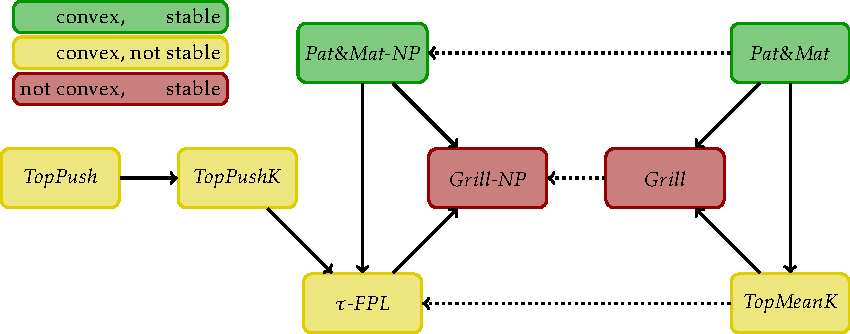
\includegraphics[width = \linewidth]{images/methods_relation.pdf}
  \caption{Summary of the formulations from Chapter~\ref{chap: framework}. Methods in green are convex, while formulations in red are non-convex. Methods in light green are vulnerable to have the global minimum at~$\bm{w}=0$. Full (dotted) arrow pointing from one formulation to another show that the latter formulation has always (usually) smaller threshold.}
  \label{fig:thresholds}
\end{figure}